\documentclass[11pt,aspectratio=1610,dvipsnames]{beamer}
\graphicspath{{figs/}}
\usetheme{default}
\usepackage{DasBeamerPaket}
\usepackage{animate}
\usepackage{lastpage}
\usepackage{tikz}
\usepackage{lmodern}
\setbeamercolor{section in toc}{fg=NavyBlue}
\setbeamercolor{frametitle}{fg=NavyBlue}
\captionsetup[figure]{labelfont=bf}
\captionsetup[table]{labelfont=bf}
\setbeamertemplate{caption}[numbered]
\title[$\Lambda(1405)$]{Experimental studies of the $\Lambda(1405)$}
\subtitle[Seminar physics654]{physics654 -- Seminar on exotic multi-quark states}

\begin{document}
\definecolor{myWhite}{rgb}{1,1,1}

\setbeamertemplate{footline}[text line]{\parbox{0.3\linewidth}{\vspace*{-9pt}\textcolor{white} \insertsection  \hfill} \parbox{0.7\linewidth}{\vspace*{-8pt} \textcolor{white}{\hfill\hspace{-3cm}\insertshorttitle \phantom{ }-- \insertshortsubtitle}  \hfill \textcolor{myWhite}{\insertpagenumber/\pageref{LastPage}}}}

\addtobeamertemplate{footline}{ \makebox[0pt][l]{\hspace{-1cm}
		\raisebox{0cm}[0pt][0pt]{\colorbox{gray!20!black}{\phantom{{\large TEXTTEXTTEXTTEXTTEXTTEXTTEXTTEXTTEXTTEXTTEXTTEXTTEXTTEXTTEXTTEXTTEXTTEXTTEXTTEXTTEXTTEXTTEXTTEXTTEXTTEXTTEXTTEXTTEXTTEXTTEXTTEXTTEXTTEXTTEXTTEXTTEXTTEXTTEXTTEXT}}}}}}

\setbeamercovered{transparent}
\setbeamertemplate{navigation symbols}{}
\setbeamertemplate{frametitle}[default][left,leftskip=0.5cm]
%
\setbeamertemplate{itemize item}{\color{black}$\blacktriangleright$}
\setbeamertemplate{section in toc}[sections numbered]
\captionsetup{font=scriptsize,labelfont=scriptsize}

\AtBeginSection[]
{	
	\definecolor{myWhite}{rgb}{0,0,0}
	\begin{frame}[noframenumbering]
		\frametitle{}
		\addtocounter{page}{-1}
		\tableofcontents[currentsection]
		
	\end{frame}
\definecolor{myWhite}{rgb}{1,1,1}
}


\begin{frame}[plain]
	\setcounter{page}{0}
	\centering
	{\Large \color{MidnightBlue}{Experimental studies of the $\Lambda(1405)$}}\\
	{\href{https://www.youtube.com/watch?v=oHg5SJYRHA0}{physics654 -- Seminar on exotic multi-quark states}}
	

	\vfill

		



			
	\textsc{Jakob Krause}\\
	\scriptsize \href{mailto:krause@hiskp.uni-bonn.de}{\faEnvelope  \hspace*{0.1cm}krause@hiskp.uni-bonn.de} {\color{black}$|$} \href{https://github.com/krausejm}{\faGithub  \hspace*{0.1cm}krausejm}\\
	
	\vspace{.5cm}
	
	Tutor: \textsc{Georg Scheluchin}\\
	 \href{mailto:scheluchin@physik.uni-bonn.de}{\faEnvelope  \hspace*{0.1cm}scheluchin@physik.uni-bonn.de}

	\vspace{0.2cm}
	
	18.06.2021
	 	
 		
\end{frame}
\section*{Motivation}
\begin{frame}{Motivation}
\begin{minipage}{\linewidth}
		\begin{tcolorbox}[colback=black!10,colframe=gray!20!black,title=What is special about the $\Lambda(1405)$?] 
			\begin{itemize}
				\item its mass does not fit well into constituent quark models which do predict baryon masses well for other baryons 
				\item invariant mass distribution (line shape) differs significantly from usual \textsc{Breit-Wigner} shapes
				\item candidate for an exotic multiquark state (bound system of $\overline{K}N$) since its mass lies just below threshold
			
 			\end{itemize}
 		\vspace{.5cm}
 		There are (very) many different theoretical approaches to explain this behavior\\
 		$\to$ There is need for more experimental data!
		\end{tcolorbox}
	{\color{red} some plots/pictures?}
\end{minipage}




	
\end{frame}
%\begin{frame}[plain]
%	\maketitle
%	\setcounter{page}{0}
%\end{frame}
\section*{Table of contents}
\begin{frame}{Table of contents}
	\tableofcontents
\end{frame}
\section{Experimental setup}
\begin{frame}{Continuous Electron Beam Accelerator Facility (CEBAF)}
	\begin{figure}
		\centering
		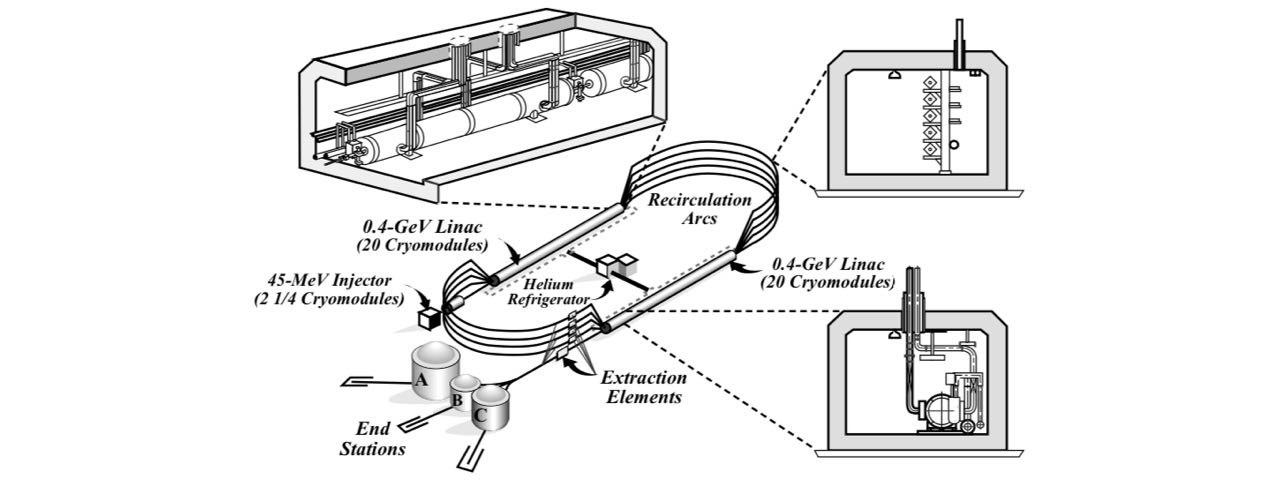
\includegraphics[width=\linewidth]{setup_big.jpg}
		\caption{CEBAF layout at Jefferson Lab, [\cite{clas}]}
	\end{figure}
\end{frame}
\begin{frame}{CEBAF Large Acceptance Spectrometer (CLAS)}
	\begin{figure}
		\centering
		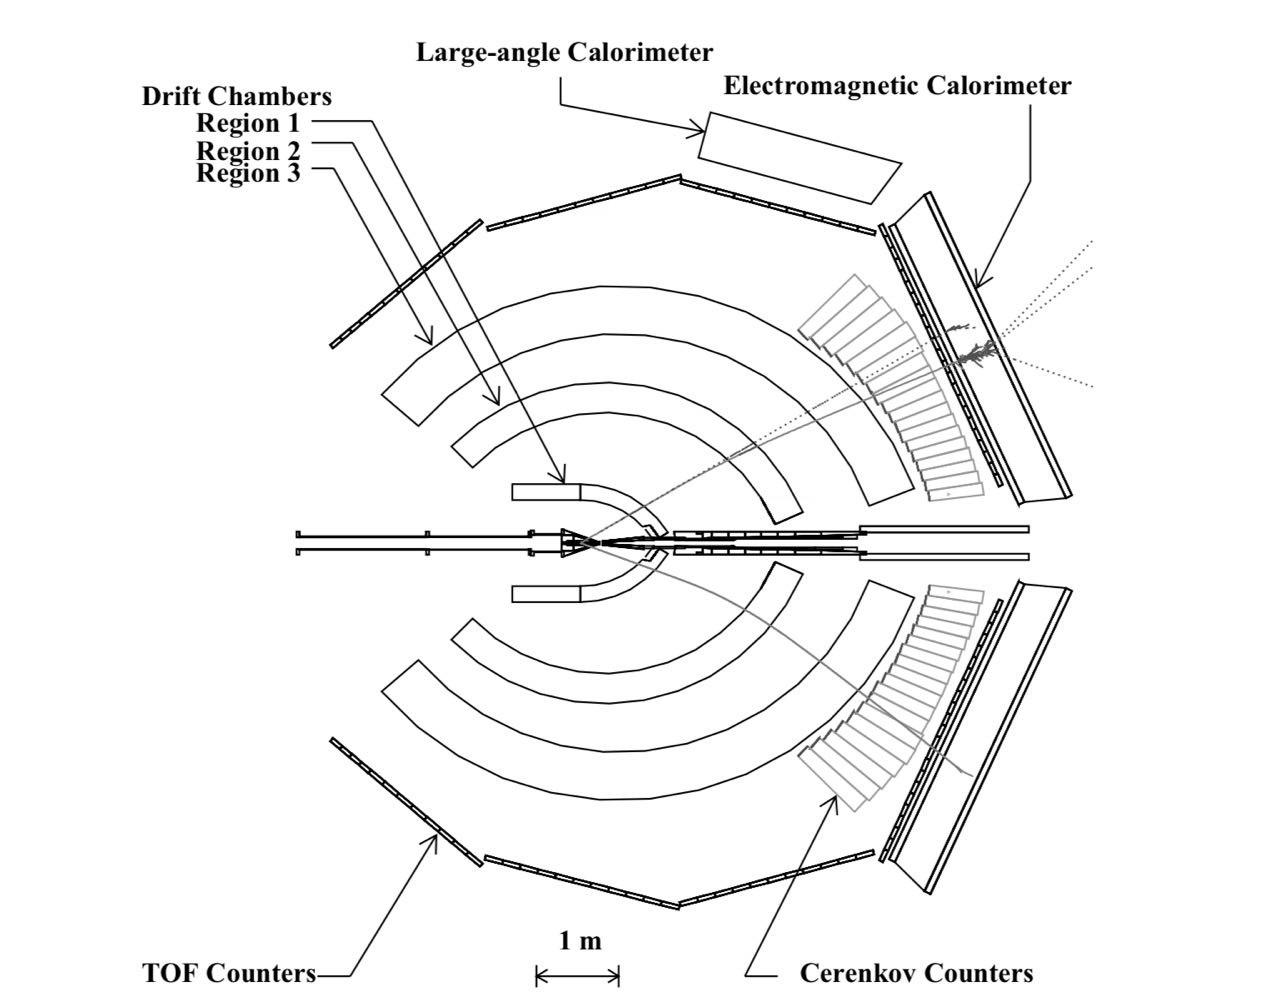
\includegraphics[width=.7\linewidth]{setup.jpg}
		\caption{CLAS layout at Jefferson Lab, [\cite{clas}]}
	\end{figure}
\end{frame}


\section{Line-shape measurement}


\begin{frame}{Reaction kinematics}
	\begin{minipage}{.65\linewidth}
		\begin{figure}[H]
			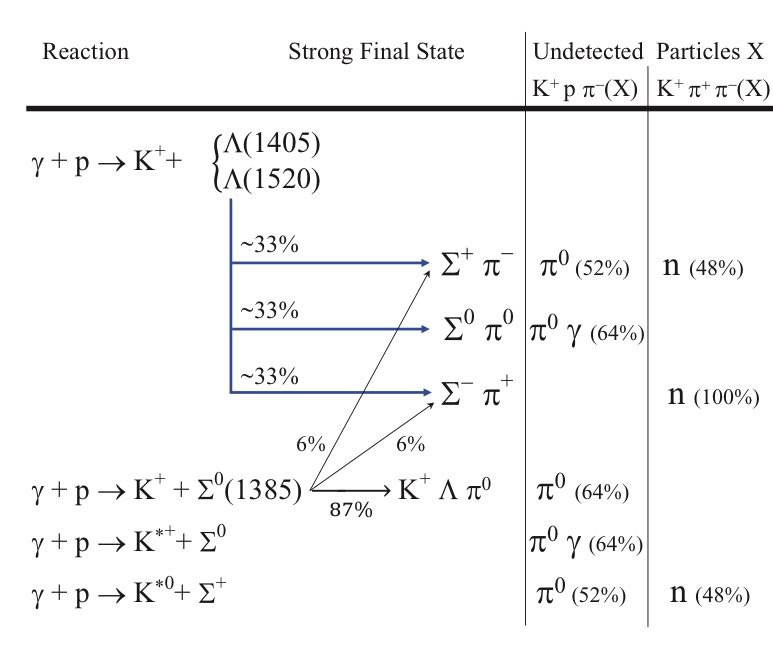
\includegraphics[width=\linewidth]{kinematics}
			\caption{Possible and studied reactions in the analysis of the lineshapes of $\Lambda(1405)$, taken from \citet{lineshapes}}
		\end{figure}	
	\end{minipage}
	\begin{minipage}{.34\linewidth}
		\begin{align*}
			\Sigma^+\to &p \pi^0\\
			\Sigma^+\to &n \pi^+\\
			\Sigma^0\to &\gamma\Lambda&\to\gamma p \pi^-\\
			\Sigma^-\to &n \pi^-\\
			\Lambda\to &p \pi^-\\
		\end{align*}
	\end{minipage}
	
\end{frame}

\begin{frame}{Event selection}
	There are two sets of reactions that the detector sees
	
	\begin{enumerate}
		\item $K^+p\pi^-$
		\item $K^+\pi^+\pi^-$
	\end{enumerate}
There are many cuts that can be made that apply to both
	\begin{tcolorbox}[colback=black!10,colframe=gray!20!black,title=Initial selection of particles] 
		\begin{itemize}
			\item Initial final state Kaon selection
			\item fiducial cuts
			\item remove false $K^+$ due to $\pi^+$ or $p$
			\item Loose $\Delta\text{TOF}$ cut ($\Delta\text{TOF}=t_\text{meas}-t_\text{calc}=t_\text{meas}-\frac{l\sqrt{p^2+m_0^2}}{cp}$)
			\item vertex $z$ cut
			\item minimum $|\mathbf{p}|$ cuts
			\item Precise $\Delta\text{TOF}$ cuts
			
		\end{itemize}
	\end{tcolorbox}
\end{frame}
\begin{frame}{Event selection}
In all channels, the data was divided into 10 bins of energy spanning \SI{100}{\mega\eV} in the CMS energy $W=\sqrt{s}$ and 20 angle bins in the CMS kaon angle.

$\to$ the following analysis was performed independently in every bin of energy and angle!
\end{frame}
\begin{frame}{Event selection}
	\centering
	\begin{minipage}{.49\linewidth}
		\begin{tcolorbox}[colback=black!10,colframe=gray!20!black,title=extracting $\Lambda\pi^0$ and $\Sigma^+\pi^-$] 
		- reminder: $\Lambda\to p\pi^-, \Sigma^+\to p\pi^0$\\	
		- final state particles: $K^+p\pi^-(\pi^0)$ 
		- determine $p_\pi$ via missing mass fit\\
		- apply cuts based on fits to the invariant masses $M_{p\pi^-}$ and $M_{p\pi^0}$	
			
			
	\end{tcolorbox}	
\end{minipage}
\begin{minipage}{.49\linewidth}
	\begin{tcolorbox}[colback=black!10,colframe=gray!20!black,title=extracting $\Sigma^+\pi^-$ and $\Sigma^-\pi^+$] 
	- reminder: $\Sigma^\pm\to n\pi^\pm$\\
	- final state particles: $K^+\pi^+\pi^-(n)$\\
	- determine $p_n$ via missing mass fit\\
	- apply cuts based on fits to the invariant masses $M_{n\pi^\pm}$
	\end{tcolorbox}	
\end{minipage}
\begin{figure}[H]
	\centering
	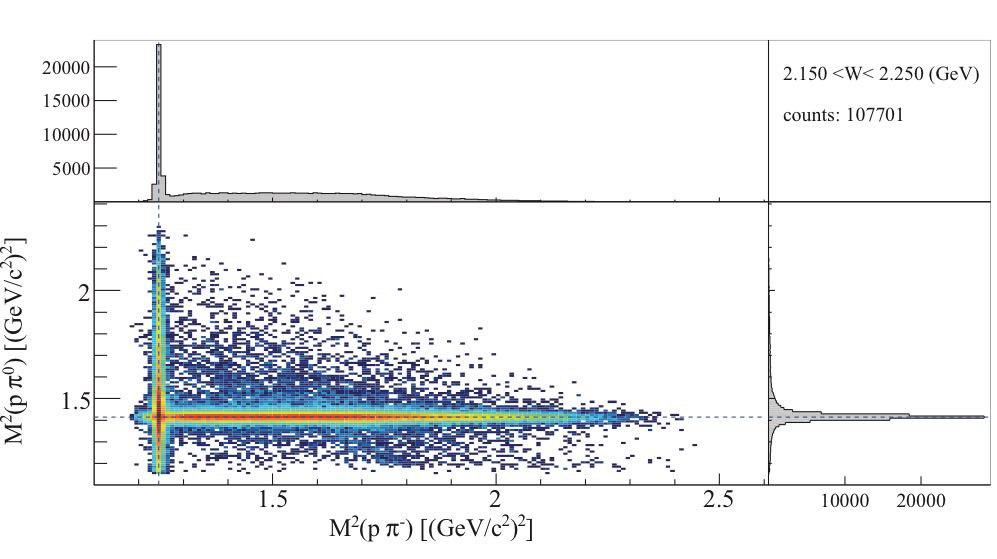
\includegraphics[width=.49\linewidth]{inv_mass_1.jpg}
	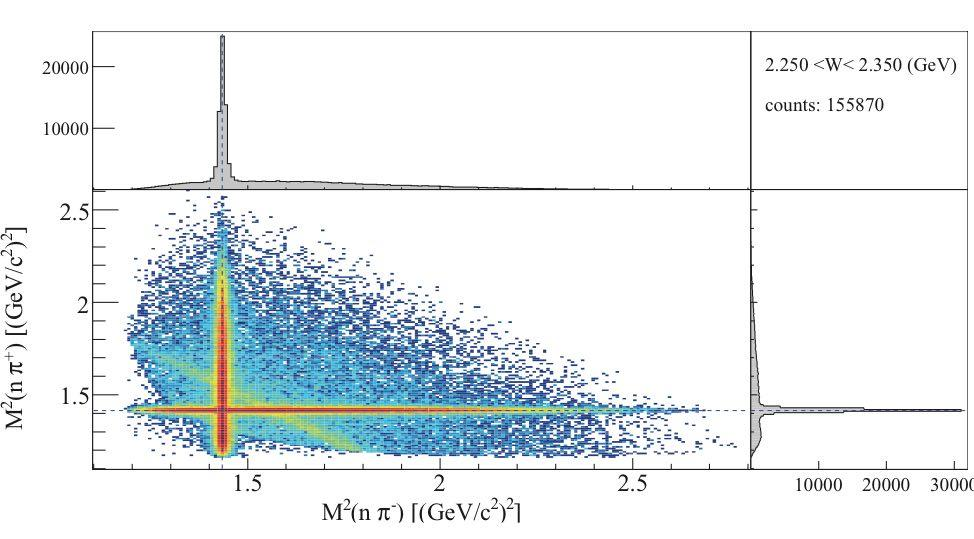
\includegraphics[width=.49\linewidth]{inv_mass_2.jpg}
	\caption{\textsc{Dalitz}-like plots of the above mentioned invariant masses, taken from \citet{lineshapes}}
\end{figure}
\end{frame}

\begin{frame}{Event selection}
	\begin{minipage}{\linewidth}
		\begin{tcolorbox}[colback=black!10,colframe=gray!20!black,title=extracting $\Sigma^0\pi^0$] 
			- reminder: $\Sigma^0\to\gamma\Lambda\to\gamma p \pi^-$\\
			- final state particles: $K^+ p \pi^-(\gamma\pi^0)$
			- missing mass fit is not applicable here: \phantom{- }demand the missing mass is sufficiently greater than $m_\pi$\\
			- make cuts based on the invariant mass $M_{p\pi^-}$\\
			- now the missing mass ($\gamma p\to K^+ X$) gives the $\Sigma^0\pi^0$ lineshape
		\end{tcolorbox}	
	\end{minipage}
\begin{figure}
	\centering
	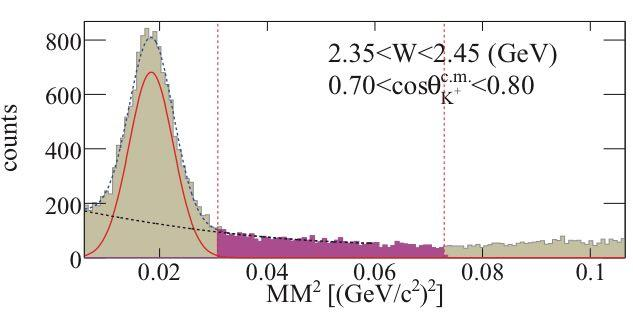
\includegraphics[width=.5\linewidth]{mism.jpg}
	\caption{Invariant mass of the $\gamma\pi$ system, selection range in magenta. Taken from \citet{lineshapes}}
\end{figure}
\end{frame}




\begin{frame}{Measurements and analysis}
	\begin{itemize}
		\item Now the signal regions have been established
		\item he true lineshape of the $\Lambda(1405)$ has to be extracted from the vast of reactions $\to$ any other contributions have to be excluded
		\item Strategy: use of \textsc{Monte-Carlo} fits to the data, simulating the contribution of other resonances
		
	\end{itemize}
\color{red} I will not really go into detail here...(??)
\end{frame}

\begin{frame}{Interpretation of the results}
	
\end{frame}





\section{Spin-parity measurement}
\begin{frame}{Theoretical basics}
	The $\Lambda(1405)$ is so far (mostly) assumed to have $J^P=\frac{1}{2}^-$, but this has not been determined experimentally
	\begin{tcolorbox}[colback=black!10,colframe=gray!20!black,title=Measuring spin] 
		\begin{itemize}
			\item consider the strong decay $Y^*\to Y\pi$, with $J^P$ the spin and parity of $Y^*$
			\item the $Y\pi$ angular distribution will only depend on $J$
			\begin{align*}
				I(\theta_Y)&=\text{const.} & J=1/2\\
				I(\theta_Y)&\propto 1+\frac{3(1-2p)}{2p+1}\cos^2\theta_Y& J=3/2,
			\end{align*}
			where $\theta_Y$ is the polar angle of the decay direction of $Y$ in the $Y^*$ rest frame, $p$ describes the fraction of spin projections along the $z$ axis 
			\item uniform decay pattern is best evidence for spin $J=1/2$
			
		\end{itemize}
	\end{tcolorbox}
	\begin{flushright}
		[\cite{spinparity}]
	\end{flushright}
	
\end{frame}
\begin{frame}{Theoretical basics}
	\begin{minipage}{.59\linewidth}
			\begin{tcolorbox}[colback=black!10,colframe=gray!20!black,title=Measuring parity] 
			\begin{itemize}
				\item the key to accessing the parity lies in determining the Polarization transfer to the decay product $Y$ which we will denote $\mathbf{Q}$
				\item the angular distribution of $\mathbf{Q}$ will only depend on $\mathbf{P}$
				\begin{align*}
				\mathbf{Q}(\theta_Y)&=\text{const.} & J^P=1/2^-\\
				\mathbf{Q}(\theta_Y)&=-\mathbf{P}+2(\mathbf{P}\cdot \mathbf{q})\mathbf{q} & J^P=1/2^+
				\end{align*}
				
				\item $\mathbf{Q}$ can be measured from weak decay angular distribution of  $Y$ 
				
			\end{itemize}
		\end{tcolorbox}		
	\end{minipage}
\begin{minipage}{.4\linewidth}
	\begin{figure}[H]
		\centering
		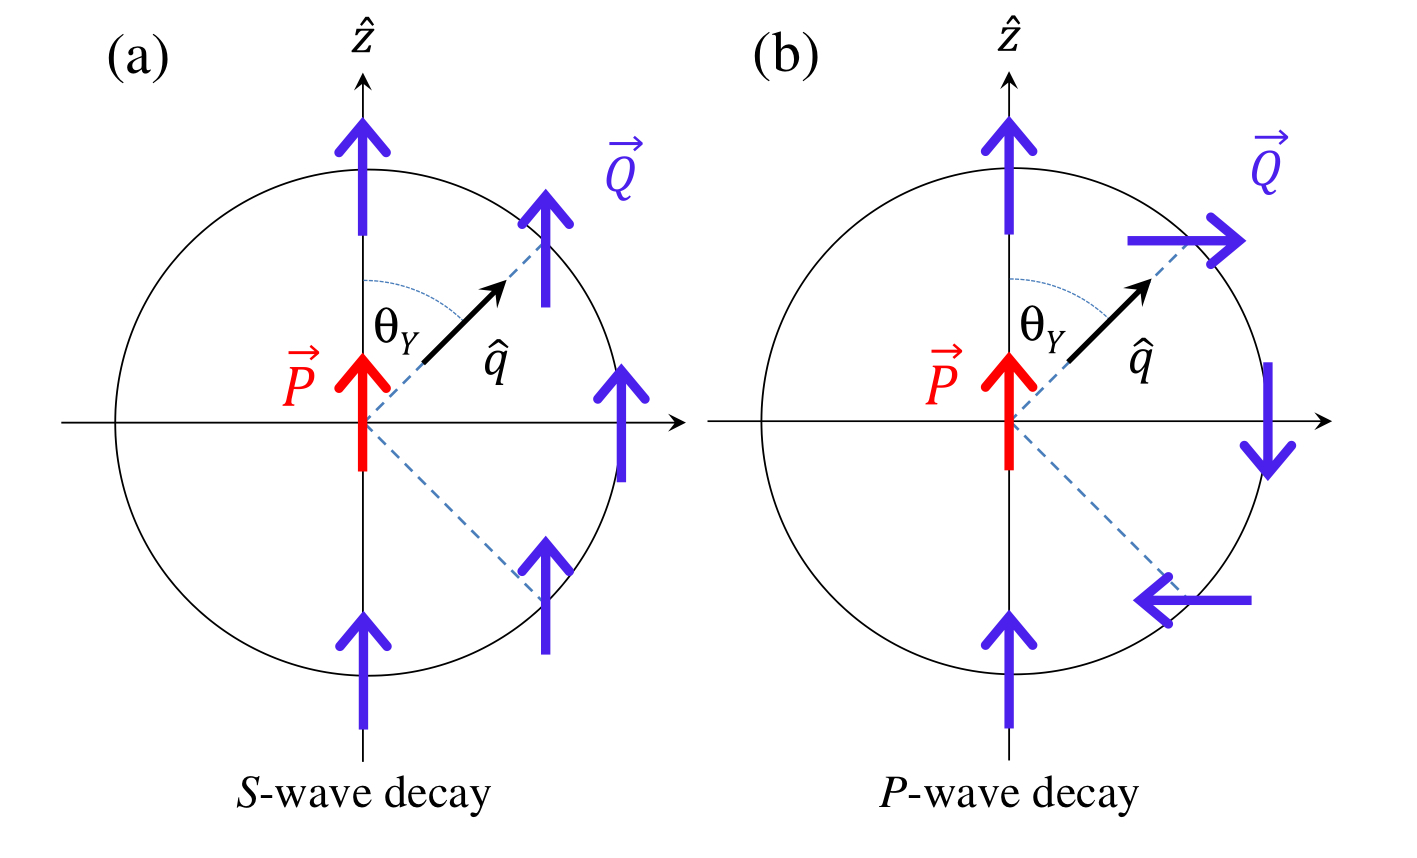
\includegraphics[width=\linewidth]{pol}
		\caption{Polarization transfer in the strong decay $Y^*\to Y\pi$, taken from [\cite{spinparity}]}
	\end{figure}
\end{minipage}

	\begin{flushright}
		[\cite{spinparity} and Ref. therein]
	\end{flushright}
\end{frame}
\begin{frame}{Measurements and analysis}
	\begin{minipage}{.4\linewidth}
			\begin{tcolorbox}[colback=black!10,colframe=gray!20!black,title=Event selection] 
			\begin{itemize}
				\item select kinematic region where the $\Sigma\pi$ invariant mass is dominated by the $\Lambda(1405)$ $\to M_{\Sigma\pi}\in$ \SIrange{1.30}{1.45}{\giga\eV}
				\item inspect nine bins in energy and angle, namely with CM energy at $2.6, 2.7$ and $2.8$ GeV and the  three forwardmost kaon angle bins each
			\end{itemize}
		\end{tcolorbox}	
\end{minipage}
\begin{minipage}{.57\linewidth}
	\begin{figure}
		\centering
		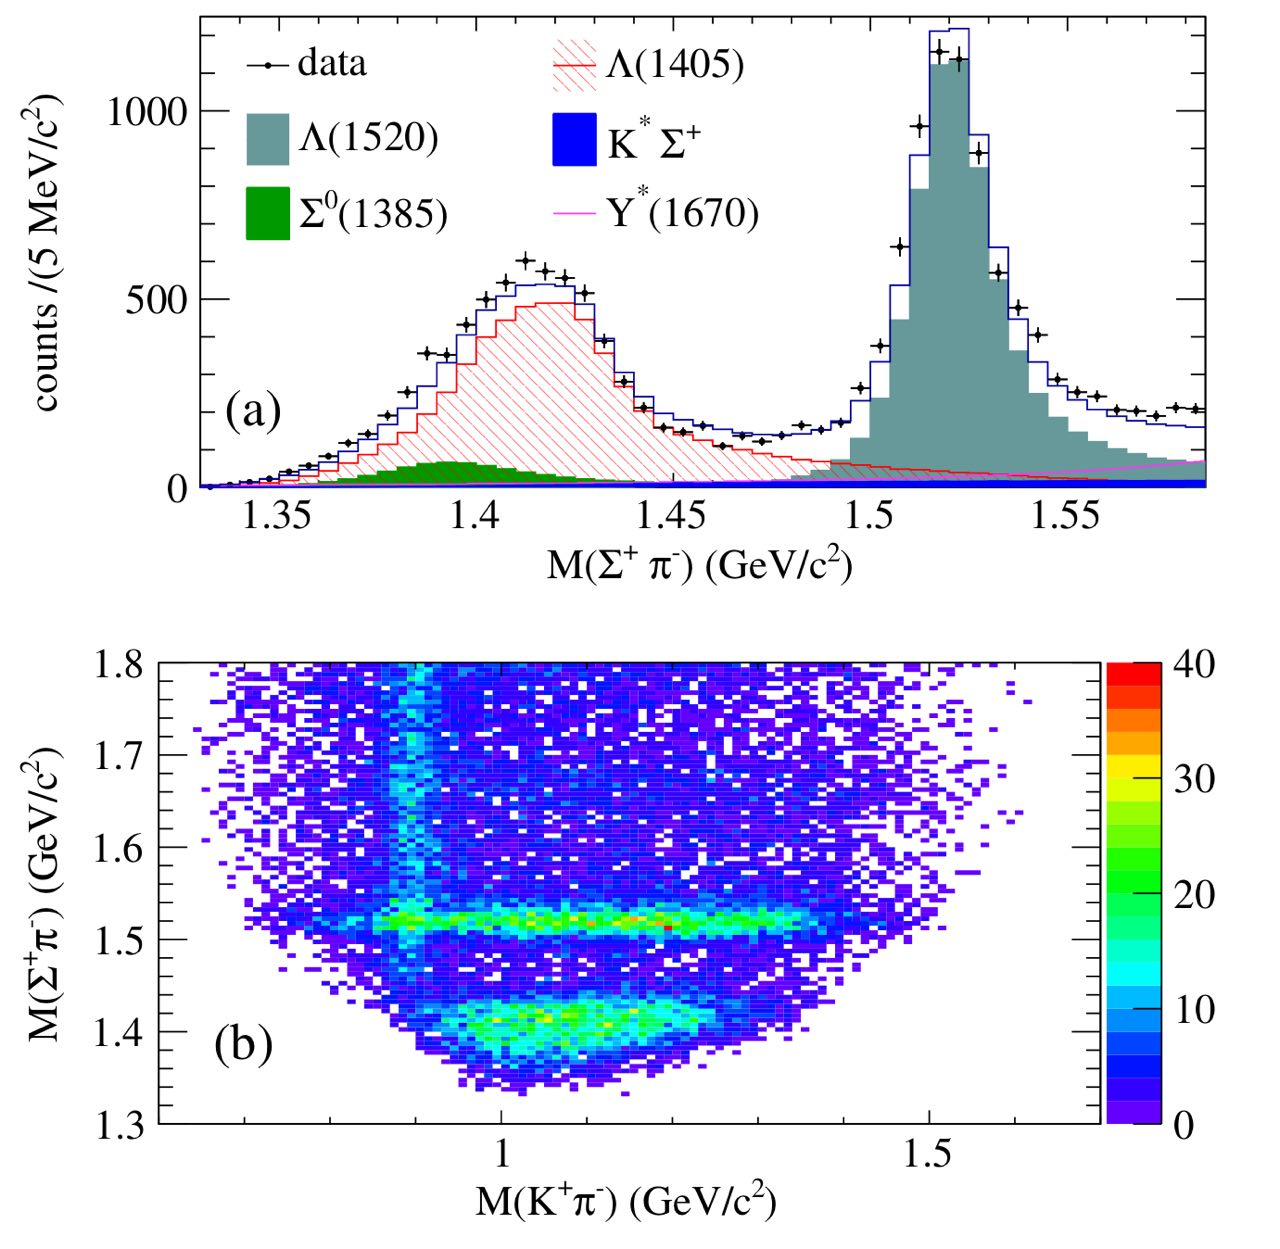
\includegraphics[width=.95\linewidth]{events_pol}
		\caption{$\Sigma\pi$  and $K\pi$ invariant mass in the vicinity of the $\Lambda(1405)$, taken from [\cite{spinparity}]}
	\end{figure}
\end{minipage}
\end{frame}
\begin{frame}{Measurements and analysis}
	\begin{minipage}{\linewidth}
	\begin{tcolorbox}[colback=black!10,colframe=gray!20!black,title=Analysis procedure] 
		\begin{itemize}
			\item plot the angular distribution of the projections  $\cos\theta_\Sigma$ and $\cos\theta_p$ for each bin
			\item test each spin hypothesis using \textsc{Monte-Carlo} maximum likelihood fits, which employ angular decay probability distributions according to each hypothesis for $\Sigma\pi$ and $p\pi$. From the fit $Q_z$ will be determined
			\item test parity hypotheses by determining $Q_z(\cos\theta_\Sigma)$
			\item compare each hypothesis by calculating a $\chi^2$ probability
		\end{itemize}
	\end{tcolorbox}	
Result: data is consistent with $J^P=1/2^-$ but does in principle not rule out $J^P=3/2^+$. $1/2^+$ and $3/2^-$ can be discarded.
\end{minipage}

\end{frame}
\begin{frame}{Measurements and analysis}
		\begin{figure}
			\centering
			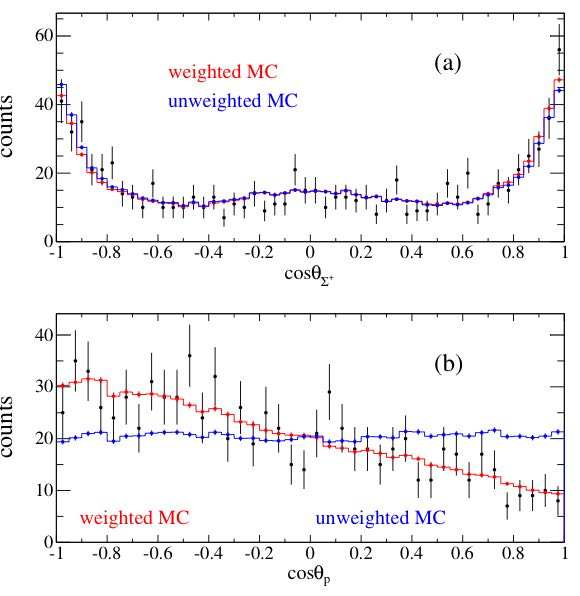
\includegraphics[width=.5\linewidth]{angular_dist}
			\caption{Distributions of the projections of (a)$\cos\theta_\Sigma$ and (b) $\cos\theta_p$ @ $2.65<W<\SI{2.75}{\giga\eV}$ and $0.70<\cos\theta<0.80$, taken from \citet{spinparity}}
		\end{figure}

\end{frame}
\begin{frame}{Measurements and analysis}
	\begin{figure}
		\centering
		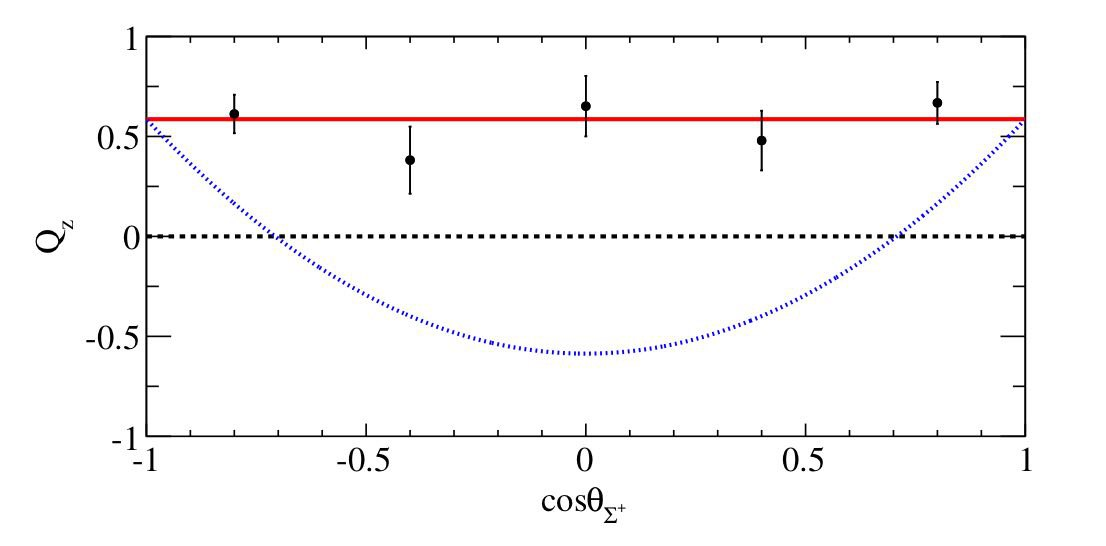
\includegraphics[width=\linewidth]{angular_pol}
		\caption{angular distribution of the polarization $Q_z$ @ $2.65<W<\SI{2.75}{\giga\eV}$ and $0.70<\cos\theta<0.80$. Red: average, blue: expectation for $P$-wave decay. Taken from \citet{spinparity}}
	\end{figure}
	
\end{frame}




\section{Conclusion}
\begin{frame}{Conclusion}
	
\end{frame}





\begin{frame}{References}
	\printbibliography
\end{frame}


\end{document}